\documentclass[10pt,aspectratio=169]{beamer}

\usetheme{Madrid}
\usecolortheme{dolphin}
\setbeamertemplate{navigation symbols}{}
\setbeamertemplate{caption}[numbered]

\usepackage[T1]{fontenc}
\usepackage[utf8]{inputenc}
\usepackage{amsmath,amssymb}
\usepackage{booktabs}
\usepackage{array}
\usepackage{tikz}
\usepackage{pgfplots}
\usepackage{listings}
\usepackage{xcolor}
\usetikzlibrary{arrows.meta,positioning,shapes.geometric,calc}
\pgfplotsset{compat=1.18}

\definecolor{mainblue}{RGB}{20,72,132}
\definecolor{accentgreen}{RGB}{36,126,92}
\definecolor{accentred}{RGB}{172,61,57}
\definecolor{lightgray}{RGB}{245,247,250}
\definecolor{codegray}{RGB}{242,244,248}

\setbeamercolor{title}{fg=white,bg=mainblue}
\setbeamercolor{frametitle}{fg=white,bg=mainblue}
\setbeamercolor{structure}{fg=mainblue}
\setbeamercolor{block title}{fg=white,bg=mainblue}
\setbeamercolor{block body}{bg=lightgray}
\setbeamercolor{alerted text}{fg=accentred}

\lstset{
  basicstyle=\ttfamily\scriptsize,
  keywordstyle=\color{mainblue}\bfseries,
  commentstyle=\color{accentgreen},
  stringstyle=\color{accentred},
  backgroundcolor=\color{codegray},
  frame=single,
  breaklines=true,
  showstringspaces=false,
  columns=fullflexible
}

\title[YuMi Cube Trajectories]{Trajectory Generation and Dual-Arm Manipulation for a YuMi Rubik's Cube Task}
\subtitle{ROS 2 control architecture, perception, scanning, handoff, and primitive execution}
\author{RVAI Homework 7 -- \texttt{yumi\_cube}}
\institute{Academic scientific presentation}
\date{\today}

\newcommand{\R}{\mathbb{R}}
\newcommand{\pose}{\mathbf{x}}
\newcommand{\quat}{\mathbf{q}}

\begin{document}

\begin{frame}
  \titlepage
\end{frame}

\begin{frame}{Outline}
  \tableofcontents
\end{frame}

\section{System Overview}

\begin{frame}{Project Goal}
  \begin{block}{Objective}
    Control a dual-arm ABB YuMi robot in simulation to localize, grasp, scan, transfer, and reorient a cube through a sequence of Rubik-style manipulation primitives.
  \end{block}

  \vspace{0.2cm}
  \begin{columns}[T]
    \begin{column}{0.48\textwidth}
      \textbf{Main capabilities}
      \begin{itemize}
        \item ROS 2 finite-state control node.
        \item Depth-based cube pose estimation.
        \item Cartesian and joint-space trajectory execution.
        \item Dual-arm cube handoff.
        \item Queue-based primitive execution.
      \end{itemize}
    \end{column}
    \begin{column}{0.48\textwidth}
      \textbf{Trajectory emphasis}
      \begin{itemize}
        \item Blended Cartesian paths.
        \item Polynomial time laws of degree 3, 5, or 7.
        \item Quaternion SLERP for orientation.
        \item Joint interpolation with settle checks.
      \end{itemize}
    \end{column}
  \end{columns}
\end{frame}

\begin{frame}{Software Architecture}
  \centering
  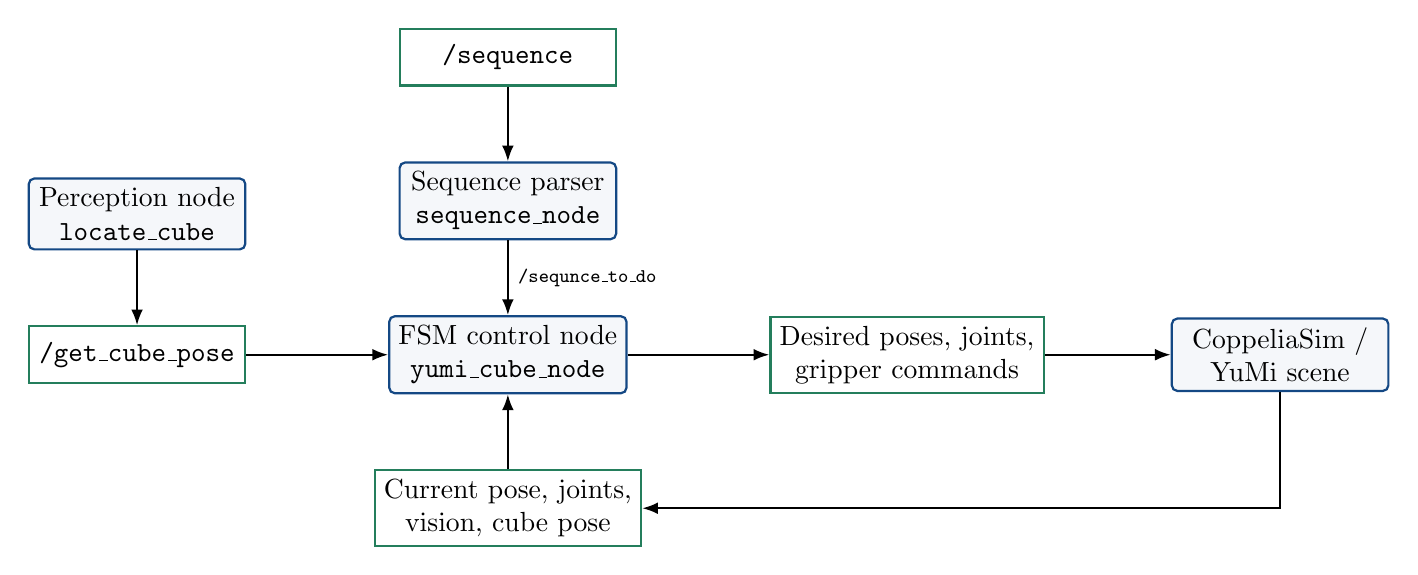
\begin{tikzpicture}[
    node distance=0.95cm and 1.1cm,
    box/.style={rectangle, rounded corners=2pt, draw=mainblue, thick, align=center, minimum width=2.75cm, minimum height=0.85cm, fill=lightgray},
    topic/.style={rectangle, draw=accentgreen, thick, align=center, minimum width=2.75cm, minimum height=0.72cm, fill=white},
    arrow/.style={-{Latex[length=2mm]}, thick}
  ]
    \node[box] (perception) {Perception node\\\texttt{locate\_cube}};
    \node[topic, below=of perception] (getpose) {\texttt{/get\_cube\_pose}};
    \node[box, right=1.8cm of getpose] (fsm) {FSM control node\\\texttt{yumi\_cube\_node}};
    \node[box, above=of fsm] (seq) {Sequence parser\\\texttt{sequence\_node}};
    \node[topic, above=of seq] (sequence) {\texttt{/sequence}};
    \node[topic, right=1.8cm of fsm] (cmds) {Desired poses, joints,\\gripper commands};
    \node[box, right=1.6cm of cmds] (sim) {CoppeliaSim /\\YuMi scene};
    \node[topic, below=of fsm] (feedback) {Current pose, joints,\\vision, cube pose};

    \draw[arrow] (perception) -- (getpose);
    \draw[arrow] (getpose) -- (fsm);
    \draw[arrow] (sequence) -- (seq);
    \draw[arrow] (seq) -- node[right, font=\scriptsize] {\texttt{/sequnce\_to\_do}} (fsm);
    \draw[arrow] (fsm) -- (cmds);
    \draw[arrow] (cmds) -- (sim);
    \draw[arrow] (sim.south) |- (feedback.east);
    \draw[arrow] (feedback) -- (fsm);
  \end{tikzpicture}

  \vspace{0.25cm}
  \small The package is organized around one high-level controller, one string-to-primitive parser, and one depth-image cube localization node.
\end{frame}

\begin{frame}{ROS 2 Interfaces}
  \begin{table}
    \centering
    \small
    \begin{tabular}{p{0.31\textwidth}p{0.23\textwidth}p{0.36\textwidth}}
      \toprule
      Interface & Type & Role \\
      \midrule
      \texttt{/yumi/right/desired\_pose}, \texttt{/yumi/left/desired\_pose} & \texttt{Pose} & Cartesian end-effector commands \\
      \texttt{/yumi/right/desired\_joint\_state}, \texttt{/yumi/left/desired\_joint\_state} & \texttt{JointState} & 7-DOF joint trajectory commands \\
      \texttt{/yumi/*/current\_pose}, \texttt{/yumi/*/current\_joint\_state} & feedback & Settle checks and trajectory starts \\
      \texttt{/get\_cube\_pose} & \texttt{Pose} & Perception output for cube center and orientation \\
      \texttt{/locate\_cube/ready} & \texttt{Bool} & One-shot trigger for perception \\
      \texttt{/sequence} $\rightarrow$ \texttt{/sequnce\_to\_do} & \texttt{String}/\texttt{Int32} & Rubik move queue \\
      \bottomrule
    \end{tabular}
  \end{table}
\end{frame}

\begin{frame}{Finite-State Task Controller}
  \centering
  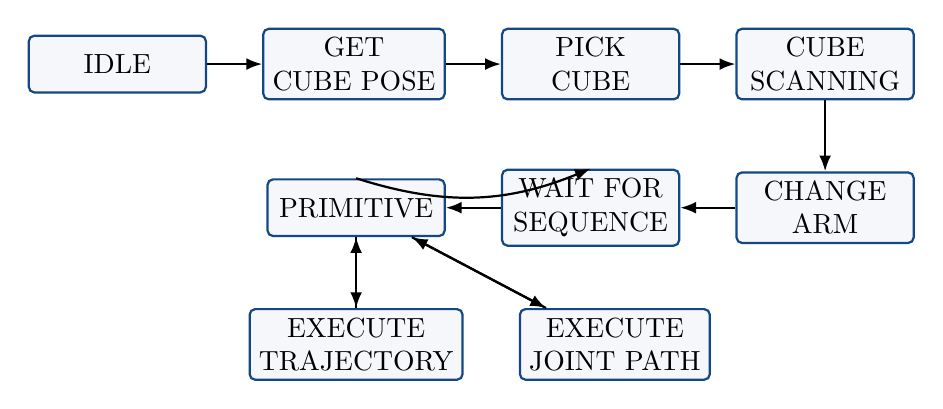
\begin{tikzpicture}[
    state/.style={rectangle, rounded corners=2pt, draw=mainblue, thick, fill=lightgray, align=center, minimum width=2.25cm, minimum height=0.72cm},
    arrow/.style={-{Latex[length=2mm]}, thick}
  ]
    \node[state] (idle) {IDLE};
    \node[state, right=0.7cm of idle] (pose) {GET\\CUBE POSE};
    \node[state, right=0.7cm of pose] (pick) {PICK\\CUBE};
    \node[state, right=0.7cm of pick] (scan) {CUBE\\SCANNING};
    \node[state, below=0.9cm of scan] (change) {CHANGE\\ARM};
    \node[state, left=0.7cm of change] (wait) {WAIT FOR\\SEQUENCE};
    \node[state, left=0.7cm of wait] (prim) {PRIMITIVE};
    \node[state, below=0.9cm of prim] (traj) {EXECUTE\\TRAJECTORY};
    \node[state, right=0.7cm of traj] (joint) {EXECUTE\\JOINT PATH};

    \draw[arrow] (idle) -- (pose);
    \draw[arrow] (pose) -- (pick);
    \draw[arrow] (pick) -- (scan);
    \draw[arrow] (scan) -- (change);
    \draw[arrow] (change) -- (wait);
    \draw[arrow] (wait) -- (prim);
    \draw[arrow] (prim) -- (traj);
    \draw[arrow] (prim) -- (joint);
    \draw[arrow] (traj) -- (prim);
    \draw[arrow] (joint) -- (prim);
    \draw[arrow] (prim.north) to[bend right=20] (wait.north);
  \end{tikzpicture}

  \vspace{0.25cm}
  \small Short multi-step actions are implemented as phase counters inside each FSM state or primitive.
\end{frame}

\section{Perception and Scanning}

\begin{frame}{Cube Pose Estimation}
  \begin{columns}[T]
    \begin{column}{0.48\textwidth}
      \textbf{Inputs}
      \begin{itemize}
        \item Depth image: \texttt{/yumi/vision\_cube/depth}
        \item Camera intrinsics: \texttt{/camera\_info}
        \item Sensor pose: \texttt{/sensor2\_pose}
        \item Far clip distance
      \end{itemize}
    \end{column}
    \begin{column}{0.48\textwidth}
      \textbf{Processing}
      \begin{itemize}
        \item Project depth pixels into a point cloud.
        \item Remove support plane by RANSAC.
        \item Isolate cube cluster by DBSCAN and size.
        \item Fit visible faces and estimate cube center.
        \item Transform local estimate to world frame.
      \end{itemize}
    \end{column}
  \end{columns}

  \vspace{0.35cm}
  \begin{equation*}
    X = \frac{(u-c_x)Z}{f_x}, \qquad
    Y = \frac{(v-c_y)Z}{f_y}, \qquad
    \mathbf{p}_{w} = R_{ws}\mathbf{p}_{s} + \mathbf{t}_{ws}.
  \end{equation*}
\end{frame}

\begin{frame}{Scanning Strategy}
  \begin{columns}[T]
    \begin{column}{0.55\textwidth}
      \begin{enumerate}
        \item Right arm holds cube at sensor view pose.
        \item Wrist joint 7 rotates by $\pi$ and returns.
        \item Right arm moves to a manually selected scan joint configuration.
        \item Cube is handed off to the left arm.
        \item Left arm performs yaw-oriented views and a second scan joint configuration.
      \end{enumerate}
    \end{column}
    \begin{column}{0.4\textwidth}
      \begin{block}{Stored scan artifacts}
        Six \texttt{256x256} RGB frames are saved in \texttt{scan\_images/}, one per selected scan phase.
      \end{block}
      \begin{block}{Trajectory relevance}
        Scanning uses both end-effector rotations at fixed position and full joint-space reconfiguration.
      \end{block}
    \end{column}
  \end{columns}
\end{frame}

\section{Trajectory Generation}

\begin{frame}{Trajectory Abstraction}
  \begin{block}{Two command spaces}
    \begin{itemize}
      \item Cartesian path: publishes \texttt{geometry\_msgs/Pose} samples to the selected arm.
      \item Joint path: publishes \texttt{sensor\_msgs/JointState} samples for seven YuMi joints.
    \end{itemize}
  \end{block}

  \vspace{0.15cm}
  \begin{columns}[T]
    \begin{column}{0.49\textwidth}
      \textbf{Cartesian state}
      \[
        \pose(t) =
        \begin{bmatrix}
          \mathbf{p}(t) \\
          \quat(t)
        \end{bmatrix},
        \quad
        \mathbf{p}(t) \in \R^3,\;\quat(t)\in SO(3).
      \]
    \end{column}
    \begin{column}{0.49\textwidth}
      \textbf{Joint state}
      \[
        \mathbf{q}(t) =
        [q_1(t),\ldots,q_7(t)]^\top \in \R^7.
      \]
    \end{column}
  \end{columns}
\end{frame}

\begin{frame}{Geometric Path Construction}
  \begin{block}{Path model}
    Cartesian paths are generated from task waypoints and then expanded into sampled segments. Intermediate corners are rounded with quadratic Bezier blends.
  \end{block}

  \begin{columns}[T]
    \begin{column}{0.52\textwidth}
      \[
        \mathbf{p}(s) =
        (1-s)\mathbf{p}_i + s\mathbf{p}_{i+1}, \qquad s\in[0,1].
      \]
      \[
        \mathbf{b}(t) =
        (1-t)^2\mathbf{p}_0
        + 2(1-t)t\mathbf{p}_1
        + t^2\mathbf{p}_2.
      \]
      The blend radius is limited by adjacent segment lengths:
      \[
        r_{\mathrm{safe}} = \min(r, d_{\mathrm{in}}/2, d_{\mathrm{out}}/2).
      \]
    \end{column}
    \begin{column}{0.44\textwidth}
      \centering
      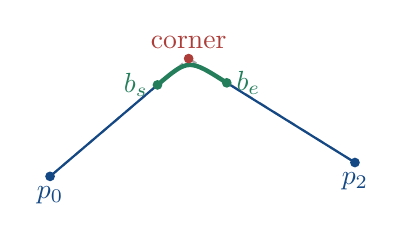
\begin{tikzpicture}[scale=0.88]
        \coordinate (A) at (0,0);
        \coordinate (B) at (2.0,1.7);
        \coordinate (C) at (4.4,0.2);
        \coordinate (S) at (1.55,1.32);
        \coordinate (E) at (2.55,1.35);
        \draw[gray!65, dashed, thick] (A) -- (B) -- (C);
        \draw[mainblue, thick] (A) -- (S);
        \draw[mainblue, thick] (E) -- (C);
        \draw[accentgreen, ultra thick] (S) .. controls (B) .. (E);
        \fill[mainblue] (A) circle (2pt) node[below] {$p_0$};
        \fill[accentred] (B) circle (2pt) node[above] {corner};
        \fill[mainblue] (C) circle (2pt) node[below] {$p_2$};
        \fill[accentgreen] (S) circle (2pt) node[left] {$b_s$};
        \fill[accentgreen] (E) circle (2pt) node[right] {$b_e$};
      \end{tikzpicture}
    \end{column}
  \end{columns}
\end{frame}

\begin{frame}{Arc-Length Parameterization}
  The sampled path is converted into cumulative arc length:
  \[
    L_0 = 0,\qquad
    L_i = L_{i-1} + \|\mathbf{p}_i-\mathbf{p}_{i-1}\|_2.
  \]

  At runtime, the time law returns a scalar progress $s(t)\in[0,1]$ and the target length is:
  \[
    L^\star(t) = s(t)L_N.
  \]

  The active segment is selected by:
  \[
    L_{i-1}\le L^\star < L_i,
    \qquad
    \alpha =
    \frac{L^\star - L_{i-1}}{L_i-L_{i-1}}.
  \]

  The commanded Cartesian position becomes:
  \[
    \mathbf{p}_{cmd}(t) =
    (1-\alpha)\mathbf{p}_{i-1}+\alpha\mathbf{p}_{i}.
  \]
\end{frame}

\begin{frame}{Polynomial Time Laws}
  \begin{columns}[T]
    \begin{column}{0.50\textwidth}
      \begin{align*}
        s_3(\tau) &= 3\tau^2 - 2\tau^3,\\
        s_5(\tau) &= 10\tau^3 - 15\tau^4 + 6\tau^5,\\
        s_7(\tau) &= 35\tau^4 - 84\tau^5 + 70\tau^6 - 20\tau^7.
      \end{align*}
      \[
        \tau = \min\left(\frac{t-t_0}{T},1\right).
      \]
      The project configuration selects degree 7 and a nominal segment duration of 6 s.
    \end{column}
    \begin{column}{0.48\textwidth}
      \centering
      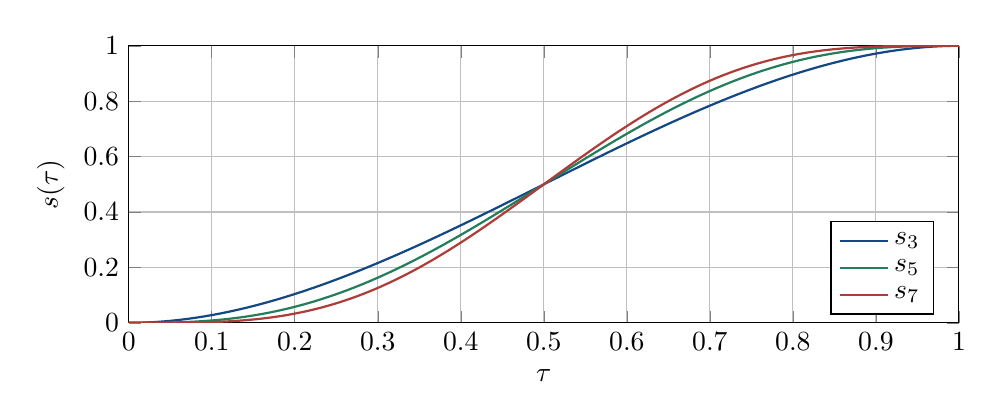
\begin{tikzpicture}
        \begin{axis}[
          width=\textwidth,
          height=5.1cm,
          xlabel={$\tau$},
          ylabel={$s(\tau)$},
          xmin=0,xmax=1,ymin=0,ymax=1,
          grid=both,
          legend pos=south east
        ]
          \addplot[mainblue, thick, domain=0:1, samples=100] {3*x^2 - 2*x^3};
          \addlegendentry{$s_3$}
          \addplot[accentgreen, thick, domain=0:1, samples=100] {10*x^3 - 15*x^4 + 6*x^5};
          \addlegendentry{$s_5$}
          \addplot[accentred, thick, domain=0:1, samples=100] {35*x^4 - 84*x^5 + 70*x^6 - 20*x^7};
          \addlegendentry{$s_7$}
        \end{axis}
      \end{tikzpicture}
    \end{column}
  \end{columns}
\end{frame}

\begin{frame}{Orientation Interpolation}
  Cartesian trajectories interpolate position along the sampled path and orientation independently by shortest-arc SLERP.

  \[
    \quat_{cmd}(t) =
    \operatorname{slerp}\left(\quat_0,\quat_f,s(t)\right).
  \]

  \begin{block}{Implementation details}
    \begin{itemize}
      \item The quaternion dot product is sign-corrected to choose the shortest rotation.
      \item Nearly parallel orientations use linear interpolation as a numerical fallback.
      \item Orientation error after execution is measured by:
      \[
        e_R = 2\cos^{-1}\left(|\quat_{actual}\cdot\quat_{cmd}|\right).
      \]
    \end{itemize}
  \end{block}
\end{frame}

\begin{frame}{Joint-Space Trajectories}
  Joint trajectories use the same scalar time law but interpolate directly in $\R^7$:
  \[
    q_i(t) =
    q_{i,0} + s(t)\left(q_{i,f}-q_{i,0}\right),
    \qquad i=1,\ldots,7.
  \]

  \begin{columns}[T]
    \begin{column}{0.48\textwidth}
      \textbf{Used for}
      \begin{itemize}
        \item Camera-pose reconfiguration.
        \item Wrist rotations during scanning.
        \item Returning arms to saved joint snapshots.
        \item Special Rubik primitive postures.
      \end{itemize}
    \end{column}
    \begin{column}{0.48\textwidth}
      \textbf{Execution checks}
      \begin{itemize}
        \item Requires current joint feedback before start.
        \item Publishes joint names \texttt{rightJoint1..7} or \texttt{leftJoint1..7}.
        \item Waits for maximum joint error below tolerance, with timeout.
      \end{itemize}
    \end{column}
  \end{columns}
\end{frame}

\begin{frame}{Trajectory Execution Loop}
  \begin{columns}[T]
    \begin{column}{0.52\textwidth}
      \begin{enumerate}
        \item Store path, target orientation, execution arm, duration, and return state.
        \item Each 20 ms timer tick computes $\tau$, $s(\tau)$, target arc length, and interpolated pose.
        \item Publish the desired pose or joint state.
        \item At $\tau=1$, compare feedback with the command.
        \item Continue publishing until settle tolerance or timeout.
      \end{enumerate}
    \end{column}
    \begin{column}{0.43\textwidth}
      \begin{block}{Default trajectory parameters}
        \begin{itemize}
          \item \texttt{duration\_sec = 6.0}
          \item \texttt{selected\_profile = 7}
          \item \texttt{cube\_size = 0.04 m}
        \end{itemize}
      \end{block}
      \begin{block}{Why settling matters}
        The FSM does not advance solely because command time elapsed; it uses feedback to reduce phase-to-phase drift.
      \end{block}
    \end{column}
  \end{columns}
\end{frame}

\section{Task-Level Trajectories}

\begin{frame}{Pick and Place Trajectory}
  \begin{columns}[T]
    \begin{column}{0.50\textwidth}
      The pick trajectory is generated from three waypoints:
      \[
        \mathbf{p}_{start}
        \rightarrow
        \mathbf{p}_{above}
        \rightarrow
        \mathbf{p}_{cube}.
      \]
      The place trajectory similarly moves:
      \[
        \mathbf{p}_{current}
        \rightarrow
        \mathbf{p}_{above,current}
        \rightarrow
        \mathbf{p}_{sensor-front}.
      \]
      The intermediate ``above'' point adds 0.10 m in world $z$ to avoid lateral collision near the cube.
    \end{column}
    \begin{column}{0.46\textwidth}
      \centering
      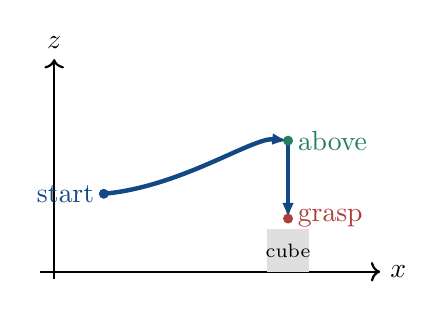
\begin{tikzpicture}[scale=0.9]
        \draw[->, thick] (-0.2,0) -- (4.6,0) node[right] {$x$};
        \draw[->, thick] (0,-0.1) -- (0,3.0) node[above] {$z$};
        \fill[gray!25] (3.0,0) rectangle (3.6,0.6);
        \node at (3.3,0.3) {\scriptsize cube};
        \coordinate (S) at (0.7,1.1);
        \coordinate (A) at (3.3,1.85);
        \coordinate (C) at (3.3,0.75);
        \draw[mainblue, ultra thick, -{Latex[length=2mm]}] (S) .. controls (1.8,1.2) and (2.8,1.9) .. (A);
        \draw[mainblue, ultra thick, -{Latex[length=2mm]}] (A) -- (C);
        \fill[mainblue] (S) circle (2pt) node[left] {start};
        \fill[accentgreen] (A) circle (2pt) node[right] {above};
        \fill[accentred] (C) circle (2pt) node[right] {grasp};
      \end{tikzpicture}
    \end{column}
  \end{columns}
\end{frame}

\begin{frame}{Dual-Arm Handoff Trajectory}
  \begin{block}{Receiver path}
    The target arm approaches the cube from a side offset mirrored by arm:
    \[
      y_{offset} =
      \begin{cases}
        +d & \text{left arm},\\
        -d & \text{right arm}.
      \end{cases}
    \]
  \end{block}

  \begin{columns}[T]
    \begin{column}{0.50\textwidth}
      \textbf{Handoff phases}
      \begin{enumerate}
        \item Open receiving gripper.
        \item Move receiver to handoff pose.
        \item Close receiver gripper.
        \item Open source gripper.
        \item Retreat source arm along mirrored $y$.
      \end{enumerate}
    \end{column}
    \begin{column}{0.46\textwidth}
      \textbf{Orientation}
      \[
        R_{receiver} \approx
        R_{source}\,R_x(\pi)\,R_z(\pm \pi/2).
      \]
      The sign is selected by closest quaternion match to the receiver reference pose, reducing unnecessary wrist motion.
    \end{column}
  \end{columns}
\end{frame}

\begin{frame}{Rubik Primitive Classes}
  \begin{table}
    \centering
    \small
    \begin{tabular}{p{0.22\textwidth}p{0.28\textwidth}p{0.38\textwidth}}
      \toprule
      Primitive class & Examples & Trajectory pattern \\
      \midrule
      Handoff rotation & R, L, R2, L2 & Ensure held arm, approach with opposite arm, rotate joint 7, restore joints \\
      Left-held upper/down moves & U, D, U2, D2 & Hold cube with left arm, move right arm in cube reference frame, wrist yaw \\
      Right-held front/back moves & F, B, F2, B2 & Reposition right arm, align left arm to right reference, wrist yaw \\
      Scene synchronization & all primitives & Publish \texttt{/cube\_cmd} to update the simulated cube state \\
      \bottomrule
    \end{tabular}
  \end{table}

  \vspace{0.15cm}
  The primitive layer composes reusable trajectory actions instead of implementing a separate low-level controller for each Rubik move.
\end{frame}

\begin{frame}{Example Primitive Sequence}
  \begin{columns}[T]
    \begin{column}{0.55\textwidth}
      A typical primitive phase sequence:
      \begin{enumerate}
        \item Save both arms' initial joint states.
        \item Move the non-holding arm through task-space approach waypoints.
        \item Align the moving wrist axis to a cube-face reference axis.
        \item Rotate joint 7 by $\pm\pi/2$ or $\pi$.
        \item Publish the matching Rubik command.
        \item Return one or both arms to their saved configurations.
      \end{enumerate}
    \end{column}
    \begin{column}{0.41\textwidth}
      \begin{block}{Local frame targeting}
        Approach points are computed by applying offsets in the held cube arm frame:
        \[
          \mathbf{p}_{target}
          =
          \mathbf{p}_{ref}
          +
          R_{ref}
          \begin{bmatrix}
          x_l\\y_l\\z_l
          \end{bmatrix}.
        \]
      \end{block}
    \end{column}
  \end{columns}
\end{frame}

\section{Evaluation and Discussion}

\begin{frame}{Trajectory Design Strengths}
  \begin{itemize}
    \item \textbf{Unified executor:} pick, scan, handoff, and primitive motions share the same time-scaling and feedback logic.
    \item \textbf{Smooth waypoint handling:} Bezier blending reduces stop-and-turn behavior at intermediate corners.
    \item \textbf{Arc-length progress:} velocity is distributed over geometric distance, not waypoint index.
    \item \textbf{Orientation continuity:} SLERP and closest-symmetric yaw avoid unnecessary wrist discontinuities.
    \item \textbf{Task robustness:} initial joint snapshots allow primitives to return arms to known configurations.
  \end{itemize}
\end{frame}

\begin{frame}{Limitations and Improvement Directions}
  \begin{itemize}
    \item Current Cartesian paths are geometric and do not explicitly enforce collision constraints beyond hand-designed waypoints.
    \item Joint-space interpolation does not account for joint velocity, acceleration, or torque limits except indirectly through duration.
    \item Primitive definitions contain hand-tuned offsets and scan configurations; automatic planning could reduce manual calibration.
    \item Perception is one-shot and uses fixed thresholds; a probabilistic estimate with uncertainty could improve grasp robustness.
    \item The sequence parser and primitive table should be checked for consistency before extending the primitive set.
  \end{itemize}
\end{frame}

\begin{frame}{Conclusion}
  \begin{block}{Summary}
    The \texttt{yumi\_cube} project implements a complete ROS 2 manipulation pipeline: perception-triggered cube localization, finite-state task sequencing, dual-arm handoff, scanning, and Rubik primitive execution.
  \end{block}

  \begin{block}{Trajectory contribution}
    The key trajectory mechanism is a reusable sampler that combines blended Cartesian geometry, polynomial time scaling, SLERP orientation interpolation, joint-space interpolation, and feedback-based settling.
  \end{block}

  \begin{block}{Scientific takeaway}
    Complex dual-arm manipulation is achieved by composing simple, verifiable trajectory primitives under an explicit state machine.
  \end{block}
\end{frame}

\begin{frame}
  \centering
  \Huge Questions
\end{frame}

\end{document}
